\section{Server Application and Modules}

For the server application itself, C++ was chosen as the implementation language for several reasons; it is extremely efficient while having access to high-level
features such as classes, it has a large selection of well-documented third party libraries and all group members had experience with either the language or C, which it
is based upon.

As it is well known that a modular code design, where each system references each other as little as possible, designing the server application in such a way
was an easy decision. It quickly became apparent that the server could logically be split into three modules: A connection module, a database module, and an \ac{api} module,
and a small amount of central code to bind these together. These modules should be created using a mix of imperative and object-oriented code, and will be described below.

\subsection{Connection Module}

The connection module will have the responsibility for any internet communication. This module should include two classes: The first is a Connection class,
which represents an open connection, and allows data to be sent and received, as well as closing the connection. Instances of this class could represent both an incoming and an outgoing
connection, though in the case of the server application, only the incoming part is relevant.

The second class is the Listener. This class should contain functionality to accept incoming connections on a given port, and make sure that an instance of the Connection class gets created
to represent the client.

Apart from these two classes, the module also should contains a framework of unbound functions to set up and stop a Listener, while taking care of any multithreading needed, so that multiple
clients can be handled concurrently. Additionally, the module needs to include several data structures, but these should not be manipulated by code outside the module, except for ServerInfo,
which may be referenced by the framework functions. A class diagram of the module's public interface can be seen in \autoref{fig:uml_connection}.

\begin{figure}[ht]
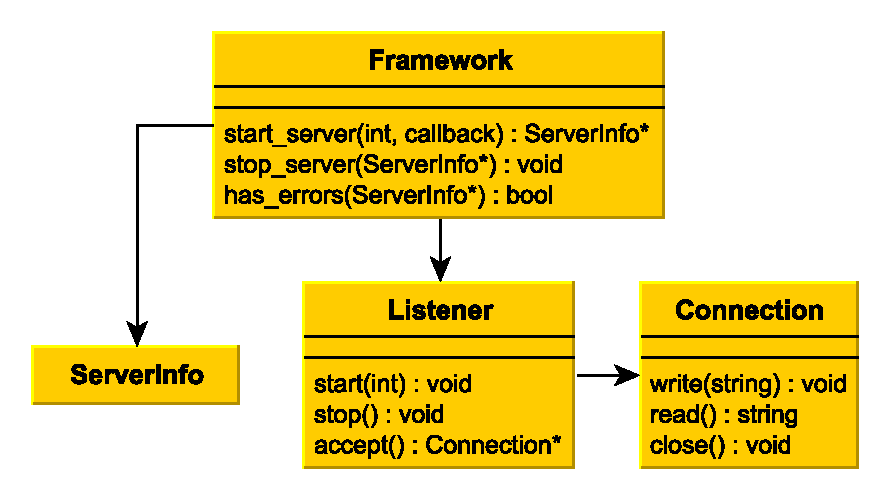
\includegraphics[scale=1]{img/connection.pdf}
\caption{Connection Class Diagram}
\label{fig:uml_connection}
\end{figure}

\subsection{Database Module}

The database module will be used to manage any connections to databases. While the actual SQL queries will be generated elsewhere in the code,
this module will be responsible for sending them and returning any results to the caller. It will contain two classes.

Instances of the first, Database, will represent a set of settings for connecting and authenticating with a database. This instance can then be used to connect to, query and escape strings for that given database.
The second class, QueryResult, is used to store whatever the database returns when queried. This result can then be read row by row. The rows should be stored in a common data type,
where each field can be accessed in any order required. A container from the C++ Standard Template Library, like a map, would be a good candidate for storing rows.
The public interface of the database module can be seen in \autoref{fig:uml_database}.

\begin{figure}[ht]
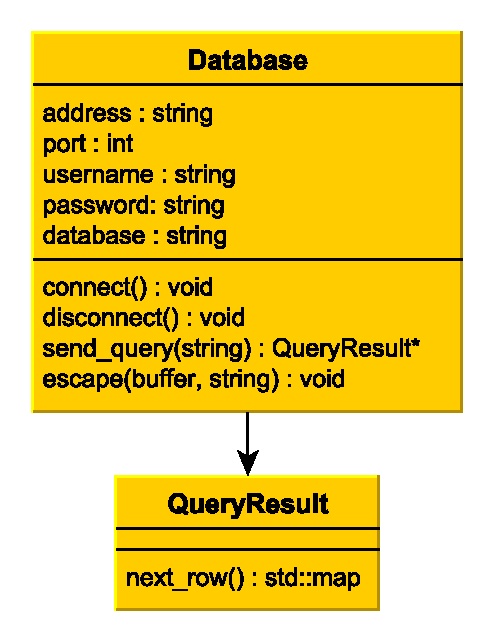
\includegraphics[scale=1]{img/database.pdf}
\caption{Database Class Diagram}
\label{fig:uml_database}
\end{figure}

\subsection{API module}

The \ac{api} module will take care of handling each request made to the server. While it is where most of the important logic happens, it is also the module with the simplest public interface, with a single class having only one public function, as seen in \autoref{fig:uml_api}.

The private interface will be much more involved however. There will be a function for each action and each data type described in the \ac{api} documentation (see Appendix \autoref{app:api}).
This creates quite a few functions, as can be seen in \autoref{fig:call_list}. Added to this will be functions to validate the structure of each type of request, as well as formatting the response and processing bulk data.
For a comprehensive overview of these helper functions, see \autoref{cha:implementation}.

\begin{figure}[ht]
\begin{tabular}[ht]{c|c|c|c|c|c|c|c|c|c|c|c|c|c|}
\cline{2-14}
&\multicolumn{2}{c|}{User}&\multicolumn{2}{c|}{Profile}&\multicolumn{2}{c|}{Dept.}&\multicolumn{2}{c|}{App.}&\multicolumn{2}{c|}{Pict.}&\multicolumn{2}{c|}{Cat.}&Misc \\
\cline{2-14}
& Li & De & Li & De & Li & De & Li & De & Li & De & Li & De & \\
\hline
\multicolumn{1}{|c|}{Read} & X & X & X & X & X & X & X & X & X & X & X & X & \\
\hline
\multicolumn{1}{|c|}{Create} & \multicolumn{2}{c|}{X} & \multicolumn{2}{c|}{X} & \multicolumn{2}{c|}{X} & \multicolumn{2}{c|}{X} &\multicolumn{2}{c|}{X} & \multicolumn{2}{c|}{X} & \\
\hline
\multicolumn{1}{|c|}{Update} & \multicolumn{2}{c|}{X} & \multicolumn{2}{c|}{X} & \multicolumn{2}{c|}{X} & \multicolumn{2}{c|}{X} &\multicolumn{2}{c|}{X} & \multicolumn{2}{c|}{X} & \\
\hline
\multicolumn{1}{|c|}{Delete} & \multicolumn{2}{c|}{X} & \multicolumn{2}{c|}{X} & \multicolumn{2}{c|}{X} & \multicolumn{2}{c|}{X} &\multicolumn{2}{c|}{X} & \multicolumn{2}{c|}{X} & \\
\hline
\multicolumn{1}{|c|}{Link} &\multicolumn{2}{c|}{}&\multicolumn{2}{c|}{}&\multicolumn{2}{c|}{}&\multicolumn{2}{c|}{}&\multicolumn{2}{c|}{}&\multicolumn{2}{c|}{}& X \\
\hline
\multicolumn{14}{l}{Note: Li = list, De = details, X = An API call to implement}
\end{tabular}
\caption{Necessary API Calls}
\label{fig:call_list}
\end{figure}

\begin{figure}[ht]
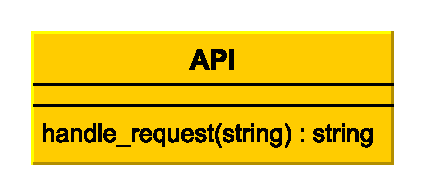
\includegraphics[scale=1]{img/api.pdf}
\caption{API Class Diagram}
\label{fig:uml_api}
\end{figure}

\subsection{Overview}

This setup results in three modules, where the only dependency will be from the \ac{api} module to the database module, as shown in \autoref{fig:uml_modules}, as the \ac{api} module is responsible for executing SQL queries, and as such needs to reference a database.
The use of callbacks in the connection library should prevent it from having any direct relation with the other modules, and while the database module could conceivably use the connection library to connect to a database,
the protocols for this communication is already implemented in the library from MySQL, which makes it easier to use the connection functionality from said library instead.

\begin{figure}[ht]
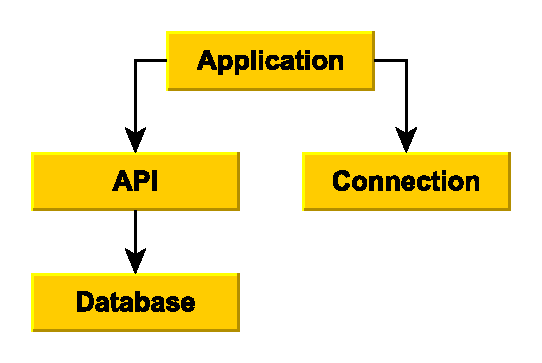
\includegraphics[scale=1]{img/modules.pdf}
\caption{Module relations}
\label{fig:uml_modules}
\end{figure}